\documentclass[12pt]{article}

\usepackage[utf8]{inputenc}

\usepackage{graphicx}

\begin{document}
%\oddsidemargin=-5mm \evensidemargin=-5mm \marginparwidth=.08in
%\marginparsep=.01in \marginparpush=5pt \topmargin=-15mm
%\headheight=12pt \headsep=25pt \footheight=12pt \footskip=30pt
%\textheight=25cm \textwidth=17cm \columnsep=2mm \columnseprule=1pt
%\parindent=15pt\parskip=2pt

\begin{center}
\bf Semestralní projekt MI-PAR 2014/2015:\\[5mm]
    Úloha DOM: i-dominující množina grafu\\[5mm]
       Tomáš Nesrovnal\\
       Adam Léhar\\[2mm]
magisterské studium, FIT ČVUT, Kolejní 550/2, 160 00 Praha 6\\[2mm]
\today
\end{center}

\section{Definice problému a popis sekvenčního algoritmu}
Naším úkolem bylo nalezení minimální i-dominující množiny W grafu G.

I-dominující množina je definována takto: Je-li dáno přirozené číslo i $\geq$ 0 a uzel u grafu G, pak i-okolí uzlu u je množina všech uzlů G ve vzdálenosti nejvýše i od u, včetně uzlu u samotného. Pak i-dominující množina grafu G je každá množina uzlů takových, že sjednocení jejich i-okolí obsahuje všechny uzly G.

Vstupem algoritmu je graf G reprezentován maticí sousednosti a hodnota i-dominance. Výstupem je počet uzlů minimální i-dominující množiny W a jejich výpis. Jednička reprezentuje uzel obsažený v množině W, nula uzel neobsažený v množině W.

Stavový prostor úlohy reprezentuje m-ární strom, kde m je počet uzlů grafu G. V hloubce k obsahuje každý uzel stromu částečné řešení obsahující k uzlů prohledávaného grafu G. Prohledávání stavového prostoru řešíme jako DFS (prohledávání grafu do hloubky). Pro urychlení výpočtu používáme metodu větví a řezů. M-ární strom reprezentující stavový prostor prořezáváme podle doposud nejlepšího nalezeného řešení. Pokud je hloubka uzlu ve stromu větší nebo rovna než počet uzlů grafu v doposud nejlepším nalezeném řešení, tak tuto větev již dále neprohledáváme protože již nemůže obsahovat zlepšující řešení. Pokud nalezneme řešení obsahující počet uzlů rovných těsné horní mezi problému, můžeme výpočet ihned ukončit. Máme zaručeno, že lepší řešení již neexistuje. Těsná horní mez je rovna $\lceil\frac{prumer(G)}{2i+1}\rceil$, kde G je graf a i je hodnota i-dominance.

\section{Popis paralelního algoritmu a jeho implementace v MPI}

Po inicializaci master procesor vygeneruje syny kořenu stromu stavového řešení a rozešle práci ostatním procesorům. Pote každý procesor vstoupí do hlavni smyčky, která se vykonává, dokud nedojde k ukončení výpočtu.

V hlavni smyčce vybírají prvky ze zásobníku a testuje se, zdali jsou, nebo nejsou řešením. Po M zpracovaných prvcích, nebo pokud nejsou prvky na zásobníku program přijme zprávy MPI a pote vyšle zprávy MPI. Nasleduje popis zprav.

Pokud procesor nalezne lepší řešení, posle ho ostatním.

Pokud procesor nemá žádnou další práci, pta se na ni postupně ostatních procesorů. Když odešle požadavek, nedělá nic jiného, než že čeká na odpověď a reaguje na přijaté zprávy. Pokud procesor dostane zadost o práci, tak pokud má dostatečný počet prvku na zásobníku, práci mu posle. Práce se posílá ve více zprávách o velikosti 950kB.

Pokud master procesoru dojde práce, kromě žádosti o práci také vyšle peška. Pešek je čistý a špinavý. Pokud nějaký procesor poslal práci procesoru s menším rankem, je špinavý. Když procesor dostane špinavého peška, pošle ho dál jako špinavého. Po odeslání peška se očistí. Když se master procesoru vrátí čistý pešek, rozešle zprávu o ukončení výpočtu. Pokud nemaster procesor dostane zprávu o ukončení výpočtu, odpoví bud ze zprávu přijal, nebo posle řešení s nejmenším počtem uzlů, pokud to byl on, co ho vypočítal.

\section{Naměřené výsledky a vyhodnocení}
Pro měření jsem si vygenerovali 3 různé grafy. Graf 1 obsahuje 200 uzlů, průměrný stupeň uzlu je 4 a i-dominance je také 4. Graf 2 obsahuje 32 uzlů, průměrný stupeň uzlu je 6 a i-dominance je 1. Graf 3 obsahuje 50 uzlů, průměrný stupeň uzlu je 3 a i-dominance je také 2.

Zrychlení na všech grafech jsme naměřili sublineární. Tento výsledek jsem očekávali, protože stejná práce je rozdělena mezi více procesorů a dále přibila komunikační režie mezi procesory. Pro graf 1 a graf 2 s 32 respektive 50 uzly dosáhl výpočet na 32 procesorech zrychlení téměř 15x. Podle grafu lze předpokládá, že zrychlení by se pro více procesorů dále zvětšovalo. Pro graf s 200 uzly na komunikační síti InfiniBand je nejlepší zrychlení pro 25 procesorů. Pak je už komunikační režie tak náročná, že dochází k poklesu zrychlení.

Pro srovnání jsem naměřili výsledky na stejných grafech také pro komunikaci přes Ethernet. Rozdíl je nejvíce patrný na grafu 1 s 200 uzly. Na rozdíl od InfiniBandu nedochází na Ethernetu k poklesu zrychlení pro více procesorů. Pro 32 procesorů jsme dosáhli zrychlení téměř 8x. Také pro další grafy jsme dosáhli lepších výsledků při komunikaci přes Ethernet. Pro graf 2 s 32 uzly je zrychlení téměř ideální, pro 32 procesorů je přibližně 31x.

\begin{table}
	\caption{Naměřené hodnoty pro graf 1: n=200, k=4, i=4}
\begin{tabular}{| l | l l l l | l l l l |}
	\hline
	 & \multicolumn{4}{c |}{InfiniBand} & \multicolumn{4}{c |}{Ethernet}\\
	\hline
	p & T(n,p) & C(n,p) & S(n,p) & E(n,p) & T(n,p) & C(n,p) & S(n,p) & E(n,p) \\
	\hline
	1 & 279.39 & 279.39 & 1.000 & 1.000 & 279.39 & 279.39 & 1.000 & 1.000 \\
	2 & 155.42 & 310.84 & 1.798 & 0.899 & 154.94 & 309.87 & 1.803 & 0.902 \\
	3 & 117.35 & 352.04 & 2.381 & 0.794 & 119.52 & 358.57 & 2.338 & 0.779 \\
	4 & 108.20 & 432.81 & 2.582 & 0.646 & 94.00 & 376.01 & 2.972 & 0.743 \\
	5 & 86.22 & 431.08 & 3.241 & 0.648 & 87.36 & 436.78 & 3.198 & 0.640 \\
	6 & 85.89 & 515.34 & 3.253 & 0.542 & 78.93 & 473.58 & 3.540 & 0.590 \\
	7 & 73.82 & 516.75 & 3.785 & 0.541 & 85.65 & 599.58 & 3.262 & 0.466 \\
	8 & 58.90 & 471.19 & 4.744 & 0.593 & 67.80 & 542.41 & 4.121 & 0.515 \\
	9 & 86.97 & 782.75 & 3.212 & 0.357 & 69.61 & 626.47 & 4.014 & 0.446 \\
	10 & 52.38 & 523.79 & 5.334 & 0.533 & 56.27 & 562.69 & 4.965 & 0.497 \\
	11 & 92.88 & 1021.72 & 3.008 & 0.273 & 60.74 & 668.12 & 4.600 & 0.418 \\
	12 & 44.61 & 535.27 & 6.263 & 0.522 & 68.27 & 819.24 & 4.092 & 0.341 \\
	13 & 84.37 & 1096.78 & 3.312 & 0.255 & 58.26 & 757.35 & 4.796 & 0.369 \\
	14 & 92.22 & 1291.08 & 3.030 & 0.216 & 60.91 & 852.70 & 4.587 & 0.328 \\
	15 & 60.29 & 904.40 & 4.634 & 0.309 & 47.80 & 716.97 & 5.845 & 0.390 \\
	16 & 60.91 & 974.51 & 4.587 & 0.287 & 47.41 & 758.62 & 5.893 & 0.368 \\
	17 & 72.92 & 1239.65 & 3.831 & 0.225 & 46.09 & 783.46 & 6.062 & 0.357 \\
	18 & 42.92 & 772.52 & 6.510 & 0.362 & 47.49 & 854.78 & 5.883 & 0.327 \\
	19 & 59.66 & 1133.53 & 4.683 & 0.246 & 45.67 & 867.74 & 6.118 & 0.322 \\
	20 & 56.78 & 1135.60 & 4.921 & 0.246 & 44.35 & 887.06 & 6.299 & 0.315 \\
	21 & 83.38 & 1750.93 & 3.351 & 0.160 & 42.45 & 891.48 & 6.581 & 0.313 \\
	22 & 52.34 & 1151.53 & 5.338 & 0.243 & 43.32 & 953.13 & 6.449 & 0.293 \\
	23 & 53.02 & 1219.38 & 5.270 & 0.229 & 42.45 & 976.46 & 6.581 & 0.286 \\
	24 & 52.55 & 1261.24 & 5.316 & 0.222 & 41.57 & 997.71 & 6.721 & 0.280 \\
	25 & 53.19 & 1329.69 & 5.253 & 0.210 & 44.19 & 1104.64 & 6.323 & 0.253 \\
	26 & 264.06 & 6865.45 & 1.058 & 0.041 & 40.32 & 1048.43 & 6.929 & 0.266 \\
	27 & 82.18 & 2218.90 & 3.400 & 0.126 & 36.73 & 991.62 & 7.607 & 0.282 \\
	28 & 255.99 & 7167.68 & 1.091 & 0.039 & 38.37 & 1074.36 & 7.281 & 0.260 \\
	29 & 260.28 & 7548.19 & 1.073 & 0.037 & 36.48 & 1058.04 & 7.658 & 0.264 \\
	30 & 274.21 & 8226.45 & 1.019 & 0.034 & 37.77 & 1133.14 & 7.397 & 0.247 \\
	31 & 269.25 & 8346.83 & 1.038 & 0.033 & 36.16 & 1120.95 & 7.727 & 0.249 \\
	32 & 265.02 & 8480.53 & 1.054 & 0.033 & 35.94 & 1150.12 & 7.774 & 0.243 \\
	\hline
\end{tabular}
\end{table}

\begin{table}
	\caption{Naměřené hodnoty pro graf 2: n=32, k=6, i=1}
\begin{tabular}{| l | l l l l | l l l l |}
	\hline
	 & \multicolumn{4}{c |}{InfiniBand} & \multicolumn{4}{c |}{Ethernet}\\
	\hline
	p & T(n,p) & C(n,p) & S(n,p) & E(n,p) & T(n,p) & C(n,p) & S(n,p) & E(n,p) \\
	\hline
	1 & 274.09 & 274.09 & 1.000 & 1.000 & 274.09 & 274.09 & 1.000 & 1.000 \\
2 & 296.87 & 593.73 & 0.923 & 0.462 & 141.90 & 283.81 & 1.932 & 0.966 \\
3 & 212.40 & 637.21 & 1.290 & 0.430 & 100.03 & 300.09 & 2.740 & 0.913 \\
4 & 144.37 & 577.47 & 1.899 & 0.475 & 68.74 & 274.96 & 3.987 & 0.997 \\
5 & 116.10 & 580.49 & 2.361 & 0.472 & 57.59 & 287.95 & 4.759 & 0.952 \\
6 & 95.85 & 575.12 & 2.859 & 0.477 & 46.79 & 280.76 & 5.858 & 0.976 \\
7 & 82.99 & 580.90 & 3.303 & 0.472 & 40.19 & 281.32 & 6.820 & 0.974 \\
8 & 74.31 & 594.46 & 3.689 & 0.461 & 35.02 & 280.15 & 7.827 & 0.978 \\
9 & 65.53 & 589.75 & 4.183 & 0.465 & 30.95 & 278.54 & 8.856 & 0.984 \\
10 & 59.55 & 595.50 & 4.603 & 0.460 & 28.06 & 280.59 & 9.769 & 0.977 \\
11 & 54.01 & 594.16 & 5.074 & 0.461 & 26.34 & 289.72 & 10.407 & 0.946 \\
12 & 50.36 & 604.29 & 5.443 & 0.454 & 23.70 & 284.36 & 11.567 & 0.964 \\
13 & 57.89 & 752.54 & 4.735 & 0.364 & 21.69 & 281.95 & 12.638 & 0.972 \\
14 & 54.26 & 759.57 & 5.052 & 0.361 & 20.13 & 281.80 & 13.617 & 0.973 \\
15 & 52.56 & 788.36 & 5.215 & 0.348 & 19.05 & 285.72 & 14.389 & 0.959 \\
16 & 39.30 & 628.82 & 6.974 & 0.436 & 18.11 & 289.80 & 15.132 & 0.946 \\
17 & 36.12 & 613.98 & 7.589 & 0.446 & 16.73 & 284.43 & 16.382 & 0.964 \\
18 & 35.27 & 634.79 & 7.772 & 0.432 & 15.88 & 285.92 & 17.255 & 0.959 \\
19 & 33.77 & 641.63 & 8.116 & 0.427 & 15.10 & 286.96 & 18.148 & 0.955 \\
20 & 32.60 & 652.09 & 8.407 & 0.420 & 14.35 & 286.92 & 19.105 & 0.955 \\
21 & 28.67 & 602.09 & 9.560 & 0.455 & 13.81 & 289.93 & 19.852 & 0.945 \\
22 & 30.14 & 663.05 & 9.094 & 0.413 & 13.21 & 290.64 & 20.747 & 0.943 \\
23 & 38.03 & 874.71 & 7.207 & 0.313 & 12.90 & 296.61 & 21.253 & 0.924 \\
24 & 28.35 & 680.36 & 9.669 & 0.403 & 12.05 & 289.14 & 22.751 & 0.948 \\
25 & 36.01 & 900.13 & 7.613 & 0.305 & 11.94 & 298.56 & 22.951 & 0.918 \\
26 & 26.03 & 676.77 & 10.530 & 0.405 & 11.40 & 296.46 & 24.038 & 0.925 \\
27 & 24.39 & 658.52 & 11.238 & 0.416 & 10.72 & 289.42 & 25.570 & 0.947 \\
28 & 24.05 & 673.50 & 11.395 & 0.407 & 10.45 & 292.47 & 26.241 & 0.937 \\
29 & 22.43 & 650.57 & 12.218 & 0.421 & 10.25 & 297.18 & 26.747 & 0.922 \\
30 & 21.13 & 633.87 & 12.972 & 0.432 & 9.98 & 299.37 & 27.467 & 0.916 \\
31 & 19.88 & 616.16 & 13.790 & 0.445 & 9.62 & 298.29 & 28.485 & 0.919 \\
32 & 18.99 & 607.71 & 14.433 & 0.451 & 8.96 & 286.61 & 30.602 & 0.956 \\
	\hline
\end{tabular}
\end{table}

\begin{table}
	\caption{Naměřené hodnoty pro graf 3: n=50, k=3, i=2}
\begin{tabular}{| l | l l l l | l l l l |}
	\hline
	 & \multicolumn{4}{c |}{InfiniBand} & \multicolumn{4}{c |}{Ethernet}\\
	\hline
	p & T(n,p) & C(n,p) & S(n,p) & E(n,p) & T(n,p) & C(n,p) & S(n,p) & E(n,p) \\
	\hline
1 & 253.28 & 253.28 & 1.000 & 1.000 & 253.28 & 253.28 & 1.000 & 1.000 \\
2 & 178.78 & 357.56 & 1.417 & 0.708 & 121.49 & 242.99 & 2.085 & 1.042 \\
3 & 119.63 & 358.88 & 2.117 & 0.706 & 82.27 & 246.81 & 3.079 & 1.026 \\
4 & 90.40 & 361.58 & 2.802 & 0.700 & 61.34 & 245.37 & 4.129 & 1.032 \\
5 & 73.02 & 365.09 & 3.469 & 0.694 & 49.69 & 248.43 & 5.098 & 1.020 \\
6 & 60.67 & 364.01 & 4.175 & 0.696 & 41.26 & 247.58 & 6.138 & 1.023 \\
7 & 52.10 & 364.70 & 4.861 & 0.694 & 35.22 & 246.52 & 7.192 & 1.027 \\
8 & 45.62 & 364.93 & 5.552 & 0.694 & 118.03 & 944.22 & 2.146 & 0.268 \\
9 & 40.53 & 364.74 & 6.250 & 0.694 & 27.40 & 246.58 & 9.245 & 1.027 \\
10 & 36.66 & 366.57 & 6.909 & 0.691 & 24.77 & 247.70 & 10.225 & 1.023 \\
11 & 33.48 & 368.31 & 7.565 & 0.688 & 22.74 & 250.18 & 11.136 & 1.012 \\
12 & 30.49 & 365.82 & 8.308 & 0.692 & 20.76 & 249.08 & 12.202 & 1.017 \\
13 & 28.68 & 372.85 & 8.831 & 0.679 & 19.29 & 250.81 & 13.128 & 1.010 \\
14 & 26.18 & 366.52 & 9.675 & 0.691 & 17.98 & 251.67 & 14.090 & 1.006 \\
15 & 25.13 & 376.94 & 10.079 & 0.672 & 60.78 & 911.67 & 4.167 & 0.278 \\
16 & 29.20 & 467.19 & 8.674 & 0.542 & 19.56 & 312.99 & 12.948 & 0.809 \\
17 & 27.64 & 469.88 & 9.164 & 0.539 & 18.84 & 320.25 & 13.445 & 0.791 \\
18 & 73.49 & 1322.77 & 3.447 & 0.191 & 18.18 & 327.27 & 13.931 & 0.774 \\
19 & 66.12 & 1256.30 & 3.831 & 0.202 & 17.51 & 332.65 & 14.466 & 0.761 \\
20 & 66.48 & 1329.61 & 3.810 & 0.190 & 16.47 & 329.36 & 15.380 & 0.769 \\
21 & 23.46 & 492.62 & 10.797 & 0.514 & 15.96 & 335.06 & 15.875 & 0.756 \\
22 & 22.86 & 503.01 & 11.078 & 0.504 & 15.55 & 342.11 & 16.287 & 0.740 \\
23 & 70.13 & 1613.00 & 3.612 & 0.157 & 14.92 & 343.22 & 16.973 & 0.738 \\
24 & 42.20 & 1012.79 & 6.002 & 0.250 & 14.53 & 348.62 & 17.436 & 0.727 \\
25 & 21.32 & 533.12 & 11.877 & 0.475 & 14.23 & 355.78 & 17.798 & 0.712 \\
26 & 38.35 & 997.13 & 6.604 & 0.254 & 13.85 & 360.11 & 18.287 & 0.703 \\
27 & 20.70 & 559.01 & 12.233 & 0.453 & 13.47 & 363.72 & 18.801 & 0.696 \\
28 & 19.69 & 551.41 & 12.861 & 0.459 & 13.38 & 374.52 & 18.936 & 0.676 \\
29 & 19.65 & 569.89 & 12.889 & 0.444 & 12.79 & 370.98 & 19.799 & 0.683 \\
30 & 19.50 & 584.97 & 12.989 & 0.433 & 38.15 & 1144.44 & 6.639 & 0.221 \\
31 & 19.22 & 595.75 & 13.179 & 0.425 & 12.40 & 384.45 & 20.423 & 0.659 \\
32 & 18.40 & 588.85 & 13.764 & 0.430 & 12.33 & 394.47 & 20.547 & 0.642 \\
	\hline
\end{tabular}
\end{table}

\begin{figure}
	\caption{Porovnání doby výpočtu s komunikací přes InfiniBand}
	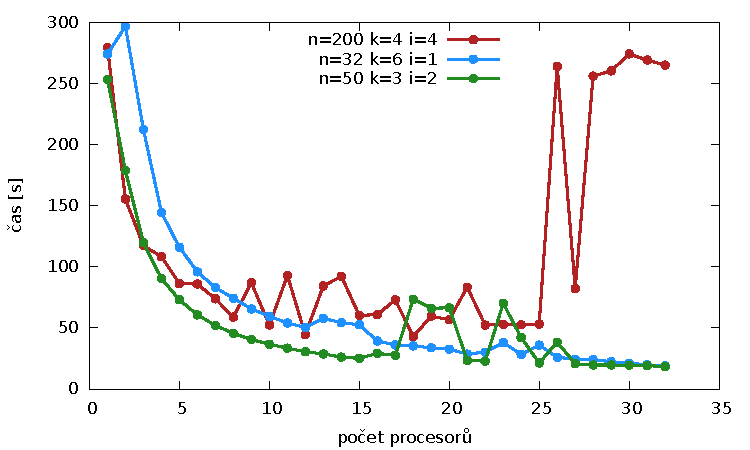
\includegraphics{graphs/time-ib.pdf}
\end{figure}

\begin{figure}
	\caption{Porovnání zrychlení s komunikací přes InfiniBand}
	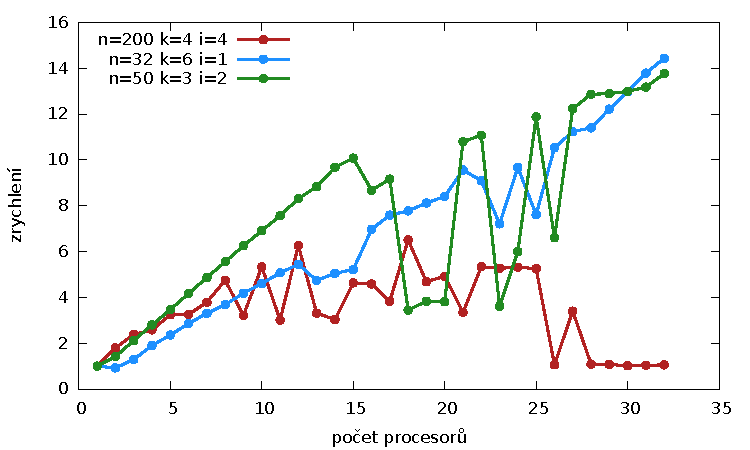
\includegraphics{graphs/speedup-ib.pdf}
\end{figure}

\begin{figure}
	\caption{Porovnání doby výpočtu s komunikací přes Ethernet}
	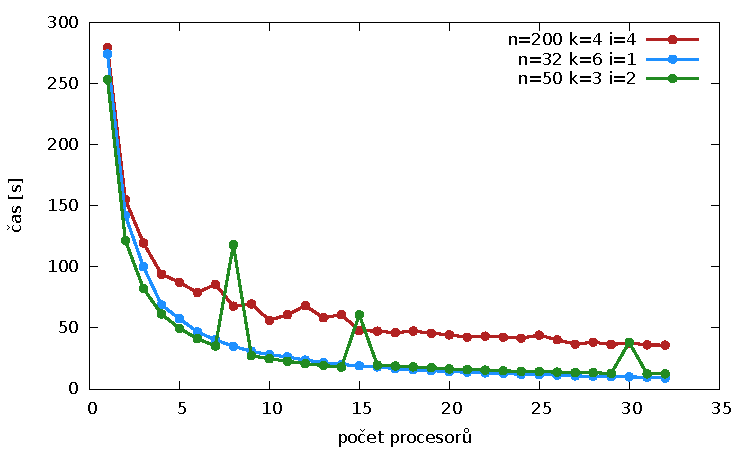
\includegraphics{graphs/time-eth.pdf}
\end{figure}

\begin{figure}
	\caption{Porovnání zrychlení s komunikací přes Ethernet}
	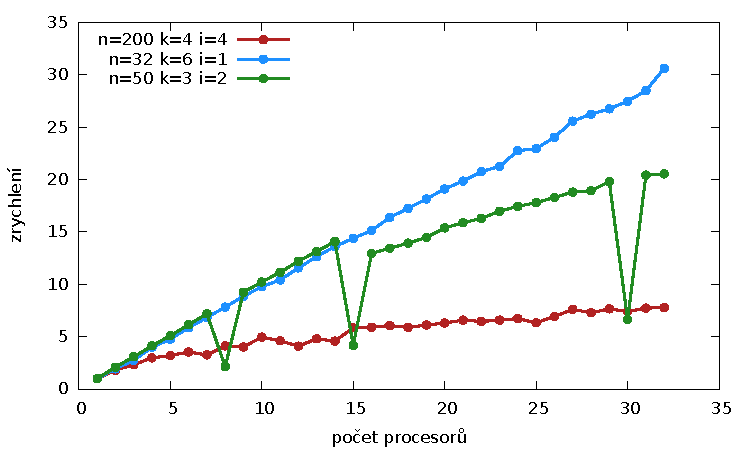
\includegraphics{graphs/speedup-eth.pdf}
\end{figure}

\begin{figure}
	\caption{Porovnání zrychlení s různými komunikačními sítěmi pro graf 1}
	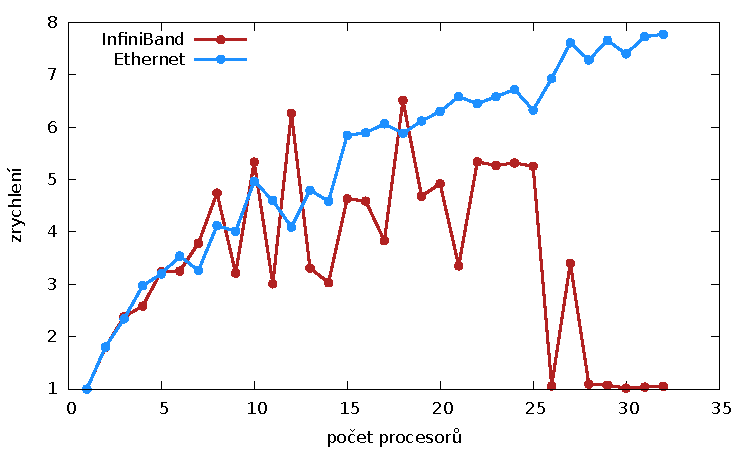
\includegraphics{graphs/graph1-speedup.pdf}
\end{figure}

\begin{figure}
	\caption{Porovnání zrychlení s různými komunikačními sítěmi pro graf 2}
	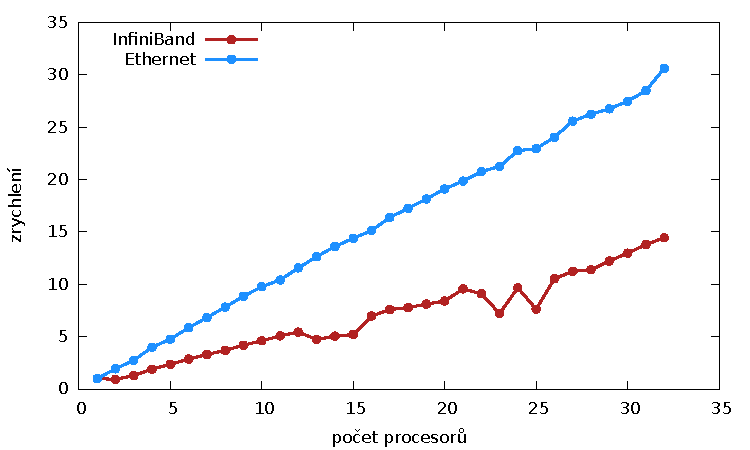
\includegraphics{graphs/graph2-speedup.pdf}
\end{figure}

\begin{figure}
	\caption{Porovnání zrychlení s různými komunikačními sítěmi pro graf 3}
	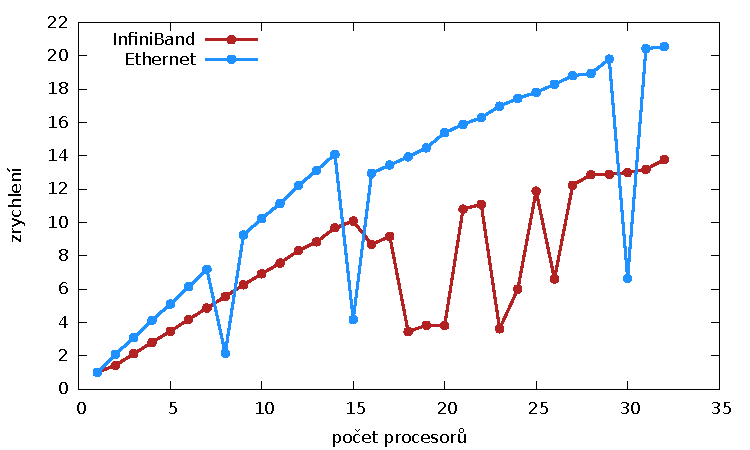
\includegraphics{graphs/graph3-speedup.pdf}
\end{figure}

\section{Závěr}
Cílem tohoto projektu bylo vyzkoušet si programování počítače s distribuovanou pamětí za pomoci knihovny MPI. Tento cíl byl úspěšně splněn a výsledkem je funkční program na výpočet minimální i-dominující množiny grafu.

Naměřené výsledky odpovídají naším předpokladům. Překvapením trochu bylo, že komunikace přes Ethernet je ve většině případů rychlejší než komunikace přes InfiniBand, která je pro takovéto systémy preferovaná.

Pro grafy s velmi hodně uzly nejsou výsledky příliš uspokojivé. Dochází zde k problémům s návrhem posílání práce ostatním procesorům. Zvolili jsme posílání pouze malých zpráv do 1kB, abychom mohli využívat blokující variantu zpráv. Při posílání velkého množství práce pak dochází k rozdělení zásobníku do více zpráv a pravděpodobně také z zahlcení komunikační sítě. S tímto fakte si lépe poradí Ethernet než InfiniBand.

Ještě lepších výsledků by šlo pravděpodobně dosáhnout předěláním posílání práce do jedné velké zprávy a tím pádem využití neblokujících variant zpráv.   

\end{document}
